\section{Relating Bipartite Matching Problem with the \texorpdfstring{$k$}{-}-SP and \texorpdfstring{$k$}{-}-SPI Problems}

\subsection{Reducing \texorpdfstring{$k$}{}-SP and \texorpdfstring{$k$}{}-SPI Problems to the Geometric Bipartite Matching Problem}\label{sec:background}
In this section, we show that the $k$-sequence partitioning problem (resp. the $k$-sequence partitioning with initial locations problem) reduces to the problem of computing a minimum-cost matching of size $n-k$ (resp. $n$) in a bipartite graph with $2n$ (resp. $2n+k$) vertices, leading to Lemma~\ref{lemma:matching-reduction}. 

% We then show that any minimum-cost $(n-k)$-partial matching on this graph corresponds to an optimal partitioning for the instance $\mcI$. We present the details in the following.

\myparagraph{Graph Representation.} Given an input sequence $\requests$ for the $k$-SP problem, recall that in our reduction, we create two vertex sets $A$ and $B$ containing $n$ points each. For each request $r_i$, we create a vertex $b_i$ (resp. $a_i$) in $B$ (resp. $A$) as the entry (resp. exit) gate for request $r_i$. The set of edges is created as follows. For any request $r_i$ and every $j > i$, we connect the exit gate $a_i$ of request $r_i$ to the entry gate $b_j$ of request $r_j$ and assign it a cost $\distance{a_i}{b_j}=\|r_i-r_j\|_p$. 
This completes the construction of the graph $\mcG_\requests$. Note that $|A|=|B|=n$.



\myparagraph{Relating a Partial Matching to a $k$-Partitioning.} 
Consider any matching $M$ of size $(n-k)$ in $\mcG_\requests$. There are exactly $k$ requests whose entry gates are free in $M$ and $k$ requests whose exit gates are free in $M$. All these requests have at most one edge incident on them. Every other request has edges incident on both the entry and exit gates. Therefore, with respect to the matching edges, $k$ requests have a degree at most one and all other requests have a degree exactly two. It is easy to see that these edges do not form a cycle, as there is no edge between the exit gate $a_i$ of a request $r_i$ to the entry gate $b_j$ of a request $r_j$ with $j<i$; therefore, the set of matching edges partitions the requests into a set of $k$ paths, representing the $k$-partitioning for the $k$-SP problem. The following lemma states and proves our reduction more formally. 

% In this part, we show that any $k$-partitioning of $\requests$ uniquely maps to a $(n-k)$-partial matching on $\mcG_\requests$ with the same cost. Similarly, we show that any $(n-k)$-partial matching on $\mcG_\requests$ uniquely maps to a $k$-partitioning of $\requests$ with the same cost. We use this observation to show that the $k$-sequence partitioning problem can be reduced to the problem of computing a minimum-cost $(n-k)$-partial matching on $\mcG_\requests$.

% Intuitively, as noted above, the points in $A$ (resp. $B$) represent the entry (resp. exit) gate of a location. Therefore, the cost of placing a request $r_i$ and a request $r_j$, for $i<j$, consecutively in a sub-sequence is represented in $\mcG_\requests$ by the edge $(b_{i}, a_{j})$. 
% We use this observation to construct a matching $M_\plan$ for each $k$-partitioning $\plan$ with the same cost by simply collecting the edges of $\mcG_\requests$ representing the consecutive requests in the sub-sequences of $\plan$. Note that for any sub-sequence $\plan_i=\langle r_{i_1}, \ldots, r_{i_t}\rangle$, the two points $b_{{i_1}}$ and $a_{{i_t}}$ are not matched in $M_\plan$, and since $\plan$ is a $k$-partitioning, the matching $M_\plan$ will be a $(n-k)$-partial matching. We also use a similar construction to show how a $(n-k)$-partial matching $M$ can be transformed to a $k$-partitioning $\plan$ with the same cost.

\begin{restatable}{lemma}{relationToMatching}\label{lemma:relationToMatching}
    Computing a minimum-cost $k$-partitioning for a sequence of requests $\requests$ reduces to computing a minimum-cost $(n-k)$-partial matching in the graph representation $\mcG_\requests$.
\end{restatable}
\begin{proof}
Consider any $k$-partitioning $\plan=\{\varsigma_1,\ldots, \varsigma_k\}$ of $\requests$. We construct a matching $M_\plan$ representing $\plan$ as follows. For any subsequence $\varsigma_i\in \plan$ and any pair of consecutive requests $r_{i_1}, r_{i_2}$ in $\varsigma_i$, we add the edge $(a_{i_1}, b_{i_2})$ to the matching $M_\plan$. Since each request $r_i\in\requests$ is included in exactly one subsequence of $\plan$, at most one edge of $M_\plan$ is incident on each point of $A\cup B$. Furthermore, for each sub-sequence $\varsigma\in\plan$, among all entry and exit gates of the requests in $\varsigma$, only the entry gate of the first request and the exit gate of the final request in $\varsigma$ are free in $M_\plan$. Hence, $M_\plan$ is a matching of size $n-k$ and by the definition of the cost of $k$-partitionings and matchings, has the same cost as $\plan$.

Next, given a $(n-k)$-partial matching $M$ on $\mcG_\requests$, we construct a $k$-partitioning $\plan_M$ of the requests $\requests$ with the same cost as $M$. Our construction relies on the following observation: since $M$ is a $(n-k)$-partial matching, all except $k$ points in $B$ are matched in $M$. For each request $r_i\in\requests$ whose entry gate $b_i$ is free in $M$, we construct a subsequence $\varsigma_i$ of requests by following the matching edges as described next. Initialize $\varsigma_i=\langle r_i\rangle$. At any step, suppose $\varsigma_i=\langle r_{i_1}, \ldots, r_{i_j}\rangle$. If the exit gate $a_{i_j}$ of the last request $r_{i_j}$ is free in $M$, we stop the construction of $\varsigma_i$; otherwise, $a_{i_j}$ is connected to an entry gate $b_{l}$ for a request $r_{l}$ with $l>i_j$. Add $r_l$ to the subsequence $\varsigma_i$ as $r_{i_{j+1}}$. This completes the construction of $k$ subsequences, one for each of the $k$ free entry gates. It is easy to confirm that the resulting subsequences are a $k$-partitioning of $\requests$ and its cost is equal to the cost of the matching $M$.
\end{proof}


\myparagraph{Extension to the $k$-SPI Problem.}
For the $k$-sequence partitioning with initial locations problem, given a sequence $\requests$ of $n$ requests and a set $\servers$ of the initial locations of the $k$ servers, we create two vertex sets $A$ and $B$, where $|A|=n+k$ and $|B|=n$. For each request $r_i\in\requests$, we create a vertex $b_i$ (resp. $a_i$) in $B$ (resp. $A$) as the entry (resp. exit) gate for request $r_i$. We also add a vertex $a^j$ for each server $s_j\in\servers$ to $A$. The set of edges is created as follows. For any server $s_j$, we add an edge from $a^j$ to the entry gate $b_i$ of all requests $r_i$ with a cost $\distance{a^j}{b_i}=\|s_j-r_i\|_p$. For any request $r_i$ and every $j > i$, we connect the exit gate $a_i$ of request $r_i$ to the entry gate $b_j$ of request $r_j$ and assign it a cost $\distance{a_i}{b_j}=\|r_i-r_j\|_p$.  See Figure~\ref{fig:enter-label}. The following lemma, whose proof is a straightforward extension of the proof of Lemma~\ref{lemma:relationToMatching}, states that the $k$-SPI problem reduces to the minimum-cost maximum matching problem on $\mcG_\requests$.

\begin{figure}
    \centering    \hspace{2em}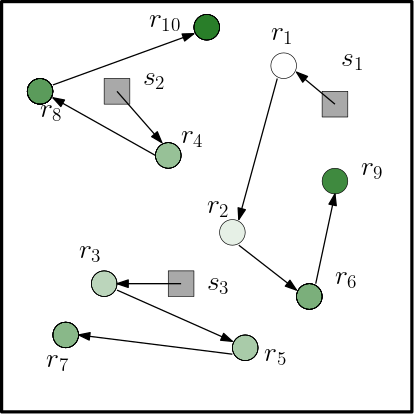
\includegraphics[width=0.4\linewidth]{figures/problem.png}\hfill
    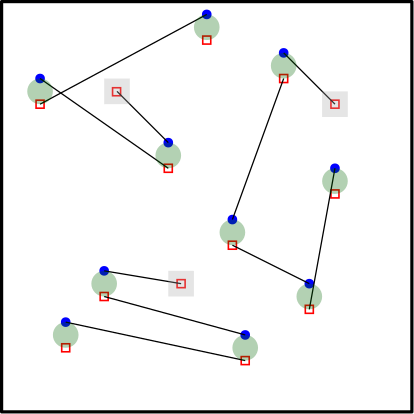
\includegraphics[width=0.4\linewidth]{figures/problem4.png}\hspace{2em}
    \caption{(Left) A $3$-partitioning $\langle s_1, r_1, r_2, r_6, r_9\rangle$, $\langle s_2, r_4, r_8, r_{10}\rangle$, $\langle s_3, r_3, r_5, r_7\rangle$ for the $3$-SPI problem and (right) its corresponding maximum matching on the graph representation of the problem.}
    \label{fig:enter-label}
\end{figure}



\begin{restatable}{lemma}{relationToMatchingServers}\label{lemma:relationToMatchingServers}
    Computing a minimum-cost $k$-partitioning with initial locations for a sequence of requests $\requests$ and a set of servers $\servers$ reduces to computing a minimum-cost maximum matching in the graph representation $\mcG_{\servers\requests}$.
\end{restatable}
\begin{proof}
For any $k$-partitioning $\plan=\{\varsigma_1,\ldots, \varsigma_k\}$ of $\requests$, we construct a matching $M_\plan$ with the same cost as follows. For any subsequence $\varsigma_i=\langle s_i, r_{i_1}, \ldots, r_{i_t}\rangle$, we add the edge $(a^i, b_{i_1})$ along with $(a_{i_j}, b_{i_{j+1}})$ for each $j\in[1, t-1]$ to $M_\plan$. Each server and each request is included in exactly one subsequence of $\plan$ and therefore, each entry gate of each request has a degree exactly one in $M_\plan$ and the exit gate of each server and each request is incident on at most one edge of $M_\plan$. Hence, $M_\plan$ is a maximum matching, and by the construction of $\mcG_\requests$, $w(M_\plan)$ is the same as the cost of $\plan$.

Next, for a maximum matching $M$ on $\mcG_\requests$, we construct a $k$-partitioning $\plan_M$ of the servers and requests $\servers\requests$ with the same cost as $M$. For each server $s_i$, we construct a subsequence $\varsigma_i$ as follows. If $a^i$ is free, then we add the subsequence $\varsigma_i=\langle s_i\rangle$ to $\plan_M$. Otherwise, $a^i$ is matched to a point $b_j$. Initialize $\varsigma_i=\langle s_i, r_j\rangle$. At any step, suppose $\varsigma_i=\langle s_i, r_{i_1}, \ldots, r_{i_j}\rangle$. If the exit gate $a_{i_j}$ of the last request $r_{i_j}$ is free in $M$, we stop the construction of $\varsigma_i$; otherwise, $a_{i_j}$ is connected to an entry gate $b_{l}$ for a request $r_{l}$ with $l>i_j$. Add $r_l$ to the subsequence $\varsigma_i$ as $r_{i_{j+1}}$. This completes the construction of $k$ subsequences, one for each of the $k$ servers. By construction, the cost of $\plan_M$ is $w(M)$.
\end{proof}



% Following that, in Section~\ref{sec:hungarian_nk}, we design a data structure that in the geometric settings the execution time of the Hungarian algorithm to $\tilde{O}(nk\Phi(n))$ time; here, $\Phi(n)$ denotes the query and update time a dynamic weighted nearest neighbor data structure. Similar improvements have been presented for complete graphs in geometric settings~\cite{agarwal1995vertical, ra_soda12, vaidya1989geometry}.   



% \paragraph{Reducing Geometric Bipartite Matching to $k$-SPI:}
% Given two sets $A=\langle a_1,\ldots, a_n\rangle$ and $B=\langle b_1,\ldots, b_n\rangle$ of $d$-dimensional points and a parameter $q\ge 1$, let $\Delta$ denote the diameter of $A\cup B$ under $\ell_q^q$ costs. We create two sets $A'$ and $B'$ of $(d+1)$-dimensional points as follows. For each point $a_i \in A$, we create a point $a_i' \in A'$ by setting the $(d+1)$st coordinate of $a_i$ to $3^{n-i+1}\Delta$. For each point $b_i \in B$, we create a point $b_i' \in B'$ and set its $(d+1)$st coordinate to $0$. Consider the $n$-SPI problem with $\servers=\langle s_1=b_1',\ldots, s_n=b_n'\rangle$ and $\requests=\langle r_1=a_1',\ldots, r_n=a_n'\rangle$ as inputs. We next show that for any $q\ge 1$, the optimal $n$-partitioning under $\ell_q^q$ norm matches each of the $n$ servers to exactly one request and the matching of servers to requests is also an optimal matching of points in $A$ to $B$. 

% \begin{figure}
%     \centering
%     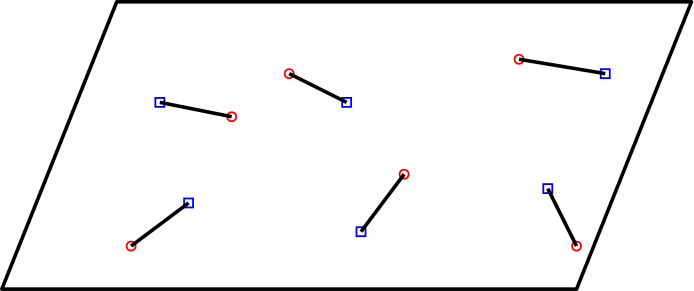
\includegraphics[width=0.45\textwidth]{figures/reduction-EBM-2.png}
%     \includegraphics[width=0.45\textwidth]{figures/reduction-EBM3-3.png}
%     \caption{(left) the point set $A$ (red points) and $B$ (blue points) and a minimum-cost bipartite matching between them, (right) the instance of $n$-SPI problem we construct from $A\cup B$.}
%     \label{fig:EBM}
% \end{figure}

% Let $\plan=\{\varsigma_1, \ldots, \varsigma_n\}$ be an optimal $n$-partitioning for $\requests'=\servers\requests$, where $\varsigma_i$ is the sub-sequence of $\requests'$ that is assigned to be served by the server $s_i$. Suppose there exists a server $s_i\in\servers$ with more than one request in $\varsigma(s_i)$, i.e., $\varsigma(s_i)=\langle s_i, r_{i_1}, \ldots, r_{i_t}\rangle$ for some $t>1$. In this case, since there are $n$ servers in $\servers$, there exists at least one server $s_j\in\servers$ with $\varsigma_j = \langle s_j\rangle$. By our construction, $\distance{s_j}{r_{i_t}}<\distance{r_{i_{t-1}}}{r_{i_t}}$. Therefore, assigning the request $r_{i_t}$ to $s_j$ reduces the cost of $\plan$, which contradicts the assumption that $\plan$ is optimal; any optimal $n$-partitioning of $\requests'$ matches each server to a single request.

% Let $\plan$ be an optimal $n$-partitioning, and for each request $r_i\in\requests$, suppose $s_{M(i)}\in\servers$ denote the server that is assigned to $r_i$ in $\plan$, where $M$ represents the matching of the servers to requests corresponding to the partitioning $\plan$. The cost of $\plan$ with $\ell_q^q$ costs is 
% \begin{align*}
%     w(\plan)&=\sum_{i=1}^n \distance{r_i}{s_{M(i)}} = \sum_{i=1}^n \distance{a'_i}{b'_{M(i)}}= \sum_{i=1}^n (3^{n-i+1}\Delta)^q + \distance{a_i}{b_{M(i)}}\\ &= \sum_{i=1}^n (3^{n-i+1}\Delta)^q + \sum_{i=1}^n \distance{a_i}{b_{M(i)}} = \sum_{i=1}^n (3^{n-i+1}\Delta)^q + w(M).
% \end{align*}

% Therefore, any algorithm that finds an optimal partitioning for the sequence partitioning problem can be used to compute a geometric bipartite matching. 

\subsection{Reducing Geometric Bipartite Matching to the \texorpdfstring{$k$}{}-SPI Problem}\label{sec:reduction}

Given an instance of the geometric bipartite matching on $d$-dimensional points $A=\{a_1,\ldots, a_n\}$ and $B=\{b_1,\ldots, b_n\}$ under the $\ell_1$ costs, we create a $(d+1)$-dimensional instance of the $k$-SPI problem. The points of $B$ will be used to create the initial locations of the $n$ servers, and the points of $A$ will be used to create the request sequence. Our construction will be such that the optimal solution to this $n$-SPI problem will create sub-sequences of length $2$ mapping the initial location of each of the $n$ servers to exactly one request. These subsequences can be shown to also correspond to the minimum-cost matching of $A$ and $B$. We provide the details below. 

Let $\diam$ denote the diameter of $A\cup B$ under $\ell_1$ costs. We create two sets $A'$ and $B'$ of $(d+1)$-dimensional points as follows. For each point $a_i \in A$, we create a point $a_i' \in A'$ by setting the $(d+1)$st coordinate of $a_i$ to $3^{n-i+1}\diam$. For each point $b_i \in B$, we create a point $b_i' \in B'$ and set its $(d+1)$st coordinate to $0$. Consider the $n$-SPI problem with $\servers=\langle s_1=b_1',\ldots, s_n=b_n'\rangle$ and $\requests=\langle r_1=a_1',\ldots, r_n=a_n'\rangle$ as inputs. By our construction, for any request $r_i$, any server $s_l$, and any request $r_j$ with $j<i$,
\begin{align}
    \|r_i- s_l\|_1 &= \|a'_i- b'_l\|_1 = 3^{n-i+1}\diam + \|a_i- b_l\|_1\le 3^{n-i+1}\diam + \diam \nonumber \\&<  (3^{n-j+1}-3^{n-i+1})\diam \le (3^{n-j+1}-3^{n-i+1})\diam + \|a_i- a_j\|_1 \nonumber \\&= \|a'_i- a'_j\|_1= \|r_i-r_j\|.\label{eq:distance-EBM}
\end{align}
Intuitively, for any request $r_i$, it would be cheaper to directly serve $r_i$ by a new server (e.g., $s_l$) rather than serving $r_i$ by a server used to serve an earlier request (e.g., $r_j$).
We next formally show that the optimal $n$-partitioning under $\ell_1$ norm matches each of the $n$ servers to exactly one request and the matching of servers to requests is also an optimal matching of points in $A$ to $B$. 

\begin{figure}
    \centering
    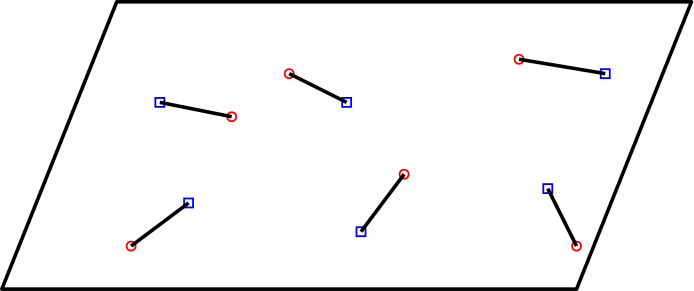
\includegraphics[width=0.45\textwidth]{figures/reduction-EBM-2.png}
    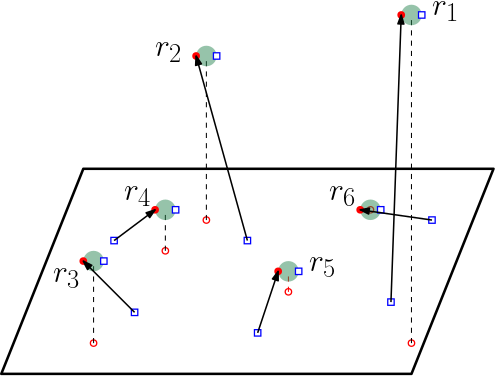
\includegraphics[width=0.45\textwidth]{figures/reduction-EBM3-4.png}
    \caption{(left) the point set $A$ (red points) and $B$ (blue points) and a minimum-cost bipartite matching between them, (right) the instance of $n$-SPI problem we construct from $A\cup B$.}
    \label{fig:EBM}
\end{figure}

Let $\plan=\{\varsigma_1, \ldots, \varsigma_n\}$ be an optimal $n$-partitioning for $\requests'=\servers\requests$, where $\varsigma_i$ is the sub-sequence of $\requests'$ that is assigned to be served by the server $s_i$. Suppose there exists a server $s_i\in\servers$ with more than one request in $\varsigma(s_i)$, i.e., $\varsigma(s_i)=\langle s_i, r_{i_1}, \ldots, r_{i_t}\rangle$ for some $t>1$. In this case, since there are $n$ servers in $\servers$, there exists at least one server $s_j\in\servers$ with $\varsigma_j = \langle s_j\rangle$. By Equation~\eqref{eq:distance-EBM}, $\|s_j-r_{i_t}\|_1<\|r_{i_{t-1}}-r_{i_t}\|_1$. Therefore, assigning the request $r_{i_t}$ to $s_j$ reduces the cost of $\plan$, which contradicts the assumption that $\plan$ is optimal; thus, any optimal $n$-partitioning of $\requests'$ matches each server to a single request.

Note that any matching $M$ of $A$ and $B$ can be used to construct an $n$-partitioning $\plan_M$ of $A'$ and $B'$. For any vertex $a_i \in A$, let $b_{m(i)}$ be its match in $M$. 
\begin{align}
    w(M)& = \sum_{i=1}^n \|a_i-b_{m(i)}\|_1=  \sum_{i=1}^n \|a_i'-b_{m(i)}'\|_1 -  3^{n-i}\diam = w(\plan_M)-\sum_{i=1}^n 3^{n-i}\diam.\label{eq:matching-EBM}
\end{align}
In other words, for any matching $M$ and $n$-partitioning $\plan_M$, the difference in the cost of $M$ and $\plan_M$ is a constant that is independent of the input. Since the optimal $n$-partitioning maps each server to a unique request and has the smallest possible cost, its corresponding matching is also a matching of $A$ and $B$ with the smallest possible cost.   
%and any $n$-partitioning $\plan_M$ of $A'$ and $B'$ where each server serves exactly one request can be used to compute a matching $M$ of $A$ and $B$. Furthermore, the difference in their $\ell_q^q$ costs is only a constant factor independent on the input. 
%\begin{align*}
%    w(\plan)& = \sum_{i=1}^n \distance{a'_i}{b'_{M(i)}}= \sum_{i=1}^n ((3^{n-i+1}\diam)^q + \distance{a_i}{b_{M(i)}})& = \sum_{i=1}^n (3^{n-i+1}\diam)^q + w(M).
%\end{align*}
%Consider any $\plan$ (not necessarily optimal) where each server serves exactly one request, and for each request $a_i'\in A'$, suppose $b_{M(i)}'\in B'$ denote the server that is assigned to $a_i'$ in $\plan$. Recollect, $a_i'$ and $b_{M(i)'}$ are constructed from $a \in A$ and $b \in B$ respectively. Let $M$ represent the matching of $A$ and $B$ where there is one edge for each subsequence in $\plan$. The cost of $\plan$ with $\ell_q^q$ costs is 
%\begin{align*}
%    w(\plan)& = \sum_{i=1}^n \distance{a'_i}{b'_{M(i)}}= \sum_{i=1}^n ((3^{n-i+1}\diam)^q + \distance{a_i}{b_{M(i)}})& = \sum_{i=1}^n (3^{n-i+1}\diam)^q + w(M).
%\end{align*}
Therefore, any algorithm that finds an optimal partitioning for the sequence partitioning problem can be used to compute a geometric bipartite matching.
Note that our reduction extends to $\ell_q^q$ distances for any parameter $q\ge 1$ in a straightforward way. 


